\chapter{Related Work}
\label{ch:problem-related-work}

As was discussed in \autoref{ch:introduction}, a common approach in \acrshort{acr:dtp} is to formulate plans by making use of (compact) probabilistic models of the systems under consideration.
In particular we focus our attention to devising \acrshort{acr:mdp} models, which need to accurately define what constitutes the state of the system, reflect uncertainty through transition probabilities, and specify goals through rewards.
The problem we face is that hand-crafting accurate, well-generalizing models is a difficult and time-costly process for a human designer.
To overcome this problem the goal is to automatize the model development process by applying learning algorithms on data that describes the stochastics of the system under consideration.
Therefore this chapter aims to provide some insight into the existing approaches for automating the development of probabilistic models for planning under uncertainty.

First \autoref{sec:learning-state-spaces} gives an overview of the existing algorithms for learning models from execution traces of the system.
Then, in \autoref{sec:active-reinforcement-learning} a number of approaches are examined, which combine offline methods for learning (initial) models with \acrshort{acr:rl} algorithms which update the model parameters online.
Subsequently, \autoref{sec:bayesian-reinforcement-learning} looks into the work that applies a technique known as Bayesian \acrlong{acr:rl} for learning models.

%\section{Problem Formulation}
%\label{sec:problem-formulation}
%
%In \acrshort{acr:dtp} it is common to make use of a (compact) probabilistic model of the environment.
%However, devising an optimal model for a specific system or process can be a daunting and error-prone task, when considering the wide range of possibilities while wanting a compact and computation-cost efficient model.

\section{Learning Probabilistic Models from Execution Traces}
\label{sec:learning-state-spaces}

\showoutline{

\noindent\textbf{Iterative Adjustment of Probabilities}:
\begin{itemize}
	\item Likelihood maximization for Markov Chains/MDPs, which generalizes to Baum-Welch for HMMs/POMDPs
	\item Bayesian Inference (see section 2.2.1)
	\item Gradient-Ascent
\end{itemize}

\begin{figure}[]
	\centering
	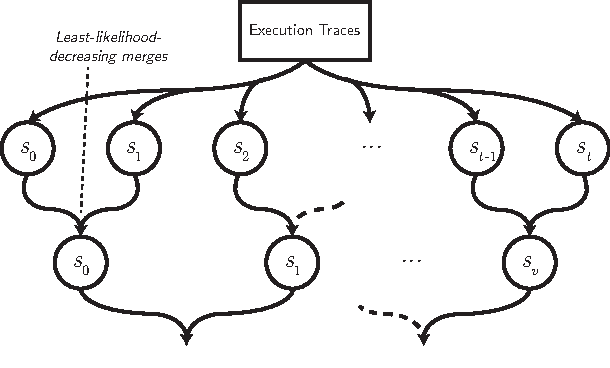
\includegraphics[width=0.8\textwidth]{model-merging-bfmm}
	\caption{State Merging (Not sure yet whether this should be here)}	% TODO
	\label{fig:state-merging}
\end{figure}

\noindent \textbf{State Merging}:
\begin{itemize}
	\item Best-First Model Merging \cite{stolcke1994best}
	\item State Merging by Trajectory Clustering \cite{nikovski2000learning}
\end{itemize}

\noindent Other approaches

}

\section{Active Reinforcement Learning}
\label{sec:active-reinforcement-learning}

\showoutline{
	\begin{itemize}
		\item Mention Model-Based \acrshort{acr:rl} or Online Model Learning
		\item Refer to approach of combining offline and online planning: using an offline-obtained model and policy, apply model-based \acrshort{acr:rl} to update the parameters \cite{epshteyn2008active}
		\item .....
	\end{itemize}
}

\section{Bayesian Reinforcement Learning}
\label{sec:bayesian-reinforcement-learning}

\showoutline{
	.....
}

% https://people.eecs.berkeley.edu/~avivt/BRLS_journal.pdf


% TODO;s
%% Fitting Markov Chains/MDPs:
	% Refer back to section 2.2.1:
	% - likelihood maximization
	% - Bayesian inference/optimization
%% Fitting HMMs/POMDPs:
	% ITERATIVE ADJUSTMENT OF PROBABILITIES:
	% - Baum-Welch Algorithm
	% - Gradient-Ascent in Likelihood
	% STATE MERGING
	% - Best-first
	% - Trajectory clustering
%% Reinforcement Learning: Online Model Learning

%% However, most of the previous works assume the state-space of the probabilistic model to be known.

%\section{Bayesian Reinforcement Learning}
%\label{sec:bayesian-reinforcement-learning}

% 

%
%\section{Overview}
%\label{sec:related-work-overview}
%
%% 